\icode{E-MM-MU-L3-260625-002}
（多选）
如图所示，光滑的水平面上有\(A\)、\(B\)、\(C\)三个物块，\(A\)、\(C\)质量均为\(m\)，\(B\)质量为\(3m\)，\(A\)、\(B\)用一根弹簧栓接并处于静止状态。某时刻，物块\(C\)以速度\(v_0\)向左运动，并与\(A\)发生碰撞，碰后\(A\)、\(C\)共速但不粘连，整个过程中，下列说法正确的是\paren[]

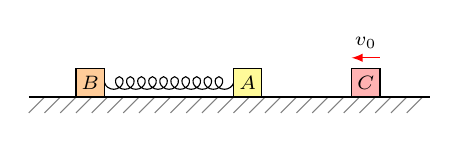
\begin{tikzpicture}[font=\scriptsize]
    \draw[decoration={aspect=1,segment length=4,amplitude=.8mm,coil},decorate](2,.18)--(.36,.18);
    \draw[fill=orange!40] (0,0) rectangle(.36,.36)node[midway,black]{\(B\)};
    \draw[fill=yellow!40] (2,0) rectangle(2.36,.36)node[midway,black]{\(A\)};
    \draw[fill=red!30] (3.5,0) rectangle(3.86,.36)node[midway,black]{\(C\)};
    \draw[red,-latex] (3.86,.5)--node[above,black]{\(v_0\)}(3.5,.5);
    \foreach \x in{-.6,-.4,...,4.4}
        \draw[gray] (\x,-.2)--++(.2,.2);
    \draw[thick] (-.6,0)--(4.5,0);
\end{tikzpicture}
\begin{choices}
    \item 弹簧的最大弹性势能为\(\frac{3mv_0^2}{20}\)
    \item 弹簧第一次恢复原长时，物块\(B\)的速度大小为\(\frac{2v_0}{5}\)
    \item 物块\(C\)的最终速度大小为\(\frac{v_0}{5}\)
    \item 弹簧最长时的弹性势能为\(\frac{3}{32}mv_0^2\)
\end{choices}
\begin{answer}
    ABD\qquad 提示：\(\Delta E_k = \frac{1}{2} \frac{m_1m_2}{m_1 + m_2}v_0\)
\end{answer}